\chapter{Methodology}
\label{chap:methodology}
This chapter develops the methodological approach for automatically performing \gls{vvuq} for automatically generated \gls{sbdt} in the manufacturing domain. The foundational methodology uses a data-driven framework and applies \gls{ml} techniques to verify and validate the \gls{sbdt}. The following chapter firstly derives requirements besides the identified key requirements given in \autoref{sec:requirements-automatically-generated-models}, categorizes them and presents a conceptual blueprint. It is based on the theoretical findings from Chapter \ref{chap:theory} and designed to ensure that the \gls{vvuq} process is systematic, reproducible, and adaptable to different use cases. It secondly describes the statistical significance testing method used to validate the results of the \gls{vvuq} process.

\section{Framework Design}
\subsection{Requirements Engineering}
An analysis of the requirements for the proposed \gls{vvuq} framework is essential. \Textcite{sindhgatta2005functional} distinguishes between \gls{fr} \textcite{van2001goal} and \gls{nfr}, \textcite{glinz2005rethinking}. Functional requirements define the specific functions and features that the system must provide, while non-functional requirements specify the quality attributes, constraints, and performance criteria that the system must possess. Additionally, \gls{tr} and \gls{or} are considered. \gls{tr} specify the technical specifications of the system which are necessary to meet the functional requirements \autocite{chikh2012new}, while \gls{or} show the operational constraints and conditions under which the system must operate \autocite{incose2023incose}.

The following \autoref{fig:requirements} summarizes the key requirements identified in \autoref{sec:requirements-automatically-generated-models} and adds requirements which have been derived from the theoretical findings in Chapter \ref{chap:theory}.

\begin{figure}[htbp]
  \centering
  
\includegraphics[width=0.8\textwidth]{figures/req.png}
  \caption[Key Requirements for VVUQ]{Key Requirements for the \gls{vvuq} framework differentiated by \gls{fr}, \gls{nfr}, \gls{tr}, and \gls{or}. }
  \caption*{Source: Authors illustration.}
  \label{fig:requirements}
\end{figure}

\gls{fr} include low-latency real-time data integration for synchronization, automatic \gls{vvuq} featuring anomaly detection, UQ, and adaptive recalibration, plus alarm management and automated \gls{kpi}-based performance evaluation. \gls{nfr} include dynamic scalability, robustness against uncertainties like noise and concept drift, security, interoperability, user-friendliness enabling easy monitoring and visualization, and continuous learning capabilities. \gls{tr} demand a scalable cloud/edge architecture supporting many data formats and protocols such as \gls{opcua} and \gls{mqtt}, integration of the ResNet \gls{bilstm} network, modules for uncertainty quantification, defined hardware resources, and data source management with quality standards. Finally, \gls{or} stresses high-standard data stewardship, continuous monitoring via logging, defined maintenance procedures, and a flexible runtime environment.

\subsection{An Automated VVUQ Framework for Automatically Generated SBDTs}
\label{sec:framework}

\begin{figure}[htbp]
  \centering
  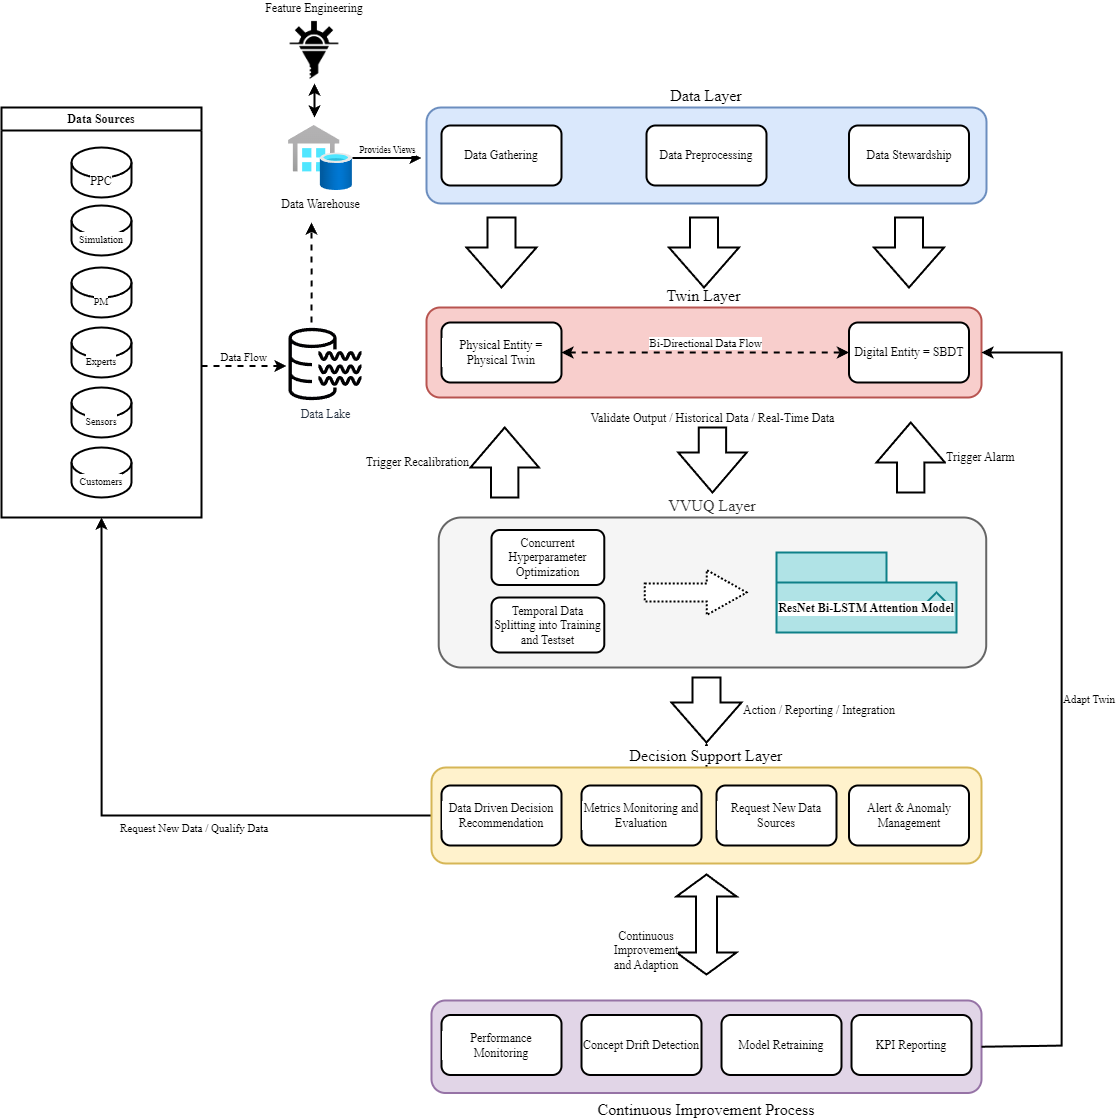
\includegraphics[width=0.8\textwidth]{figures/framework.png}
  \caption[The thesis VVUQ framework]{Framework for \gls{vvuq} of \gls{sbdt} in the manufacturing domain. The framework starts with the data sources which all lead into the data lake. The data warehouse provides the Data Layer (\gls{dl}) with different views. The \gls{dl} further enriches the data to feed it into the Twin Layer (\gls{tl}). The \gls{tl} contains the \gls{dt} and the physical entity. The \gls{tl} is connected to the \gls{vvuq} Layer (\gls{vvuql}). It incorporates the ResNet \gls{bilstm} network for \gls{vvuq} of the twin. It can trigger alarms and recommendations for action. The \gls{vvuql} is connected to the Decision Support Layer (\gls{dsl}) which provides different data analysis and visualization tools. The \gls{dsl} is responsible for the short-term decision making to manage the \gls{vvuq} process. The \gls{dsl} is connected to the user interface (\gls{ui}) which provides the user with a dashboard for monitoring and controlling the system. The \gls{dsl} can request new data from the Data Sources. It also is connected to the Continuous Improvement Process layer (\gls{cip}) which is responsible for the long-term decision making.}
  \caption*{Source: Author's illustration.}
  \label{fig:framework}
\end{figure}

The framework consists of five interconnected layers that form a closed-loop system with continuous data flow, validation and improvement. At the start, diverse data sources such as \gls{ppc} systems, \gls{des} outputs, \gls{pm}, expert knowledge, sensor networks, and \gls{crm} feedback provide the raw inputs, which are centralized in a data lake with structured views managed by a data warehouse. The data warehouse enriches the incoming data with engineering features. The \gls{dl} collects and integrates this data, preprocesses it through cleaning, normalization and feature extraction. The \gls{dl} performs a subset of the actions of the data warehouse, but tailors the data specifically for the \gls{sbdt}. This structured approach meets real-time integration and quality requirements considered above.

Within the \gls{tl}, the physical entity and its \gls{sbdt} are connected through a bi-directional data flow that ensures real-time synchronization. Evidently this framework does not allow \gls{ds} or \gls{dm}, because the closed-loop structure would be interrupted here. Complementing this, the \gls{vvuq} Layer is dedicated to the automatic \gls{vvuq} processes. This layer forms the core of the solution designed to answer how automated \gls{vvuq} can be efficiently implemented while maintaining accuracy (\autoref{par:rq1}) and determining which data-driven approaches are best suited for this task (\autoref{par:rq2}). It ensures that the \gls{sbdt} represents both the conceptual model and the physical entity, using advanced methods such as a ResNet \gls{bilstm} Attention model. The choice of this specific deep learning architecture represents the frameworks proposed answer to identifying the most suitable data-driven approaches for detecting discrepancies between simulated behaviour and real operational data (\autoref{par:rq2}). Furthermore, this DL approach, which processes historical and real-time data, provides robust anomaly detection capabilities, triggers recalibration when necessary, and validates outputs against actual measurements, thus fulfilling adaptive recalibration and anomaly detection requirements.

Translating these technical evaluations into corporate processes and recommendations is the role of the \gls{dsl}. This layer synthesizes the \gls{vvuq} assessments into prioritized \textit{short-term} decision recommendations, monitors \gls{kpi}s, identifies data gaps, and manages alerts. By serving as the interface between technical processes and operational decision-making, it ensures that manufacturing personnel receive insights. The \gls{cip} layer further enhances the system by monitoring performance, detecting concept drift, scheduling model retraining based on accumulated data, and generating \gls{kpi} reports. The \gls{cip} layer manages \textit{long-term} feedback. Through an ``Adapt Twin' process, this layer feeds insights back into the \gls{tl}, ensuring that the digital twin evolves in connection with changes in the physical entity.

\subsection{Online Validation and Continuous Feedback Loop}
\label{sec:online-validation}
The entire framework operates as a closed-loop system characterized by continuous data collection from diverse sources, real-time synchronization between physical and digital entities, ongoing validation of simulation outputs against physical measurements and a systematic flow of decision recommendations and alerts. This architecture ensures interoperability by providing standardized interfaces between layers and existing manufacturing systems while maintaining the flexibility to adapt to various manufacturing contexts. The framework transforms \gls{vvuq} from a periodic technical assessment into an ongoing process that enhances \gls{dt} quality and decision support capabilities. By meeting comprehensive functional, non-functional, technical, and operational requirements, this framework not only improves the accuracy and effectiveness of simulation-based digital twins, but also facilitates their practical application as decision support tools in modern manufacturing environments. Stakeholder feedback and personnel suggestions are integrated into the framework through the \gls{dsl} and \gls{cip} layers, ensuring that the system evolves in response to changing needs and conditions.

\section{Permutation Testing for Statistical Significance}
\label{sec:permtest}

While performance metrics such as accuracy, precision, recall, F1-score, or \gls{roc} \gls{auc} provide valuable insights into the effectiveness of a model or the magnitude of difference between datasets, they do not quantify the statistical significance of the observed results. An apparently strong performance or large difference could potentially arise due to random chance, especially with limited data or complex models. To assess whether an observed outcome is statistically significant or due to chance, permutation testing provides a robust, non-parametric approach \autocite{welch1990construction}.

Permutation testing is particularly useful when the underlying distribution of the test statistic is unknown or difficult to derive analytically, which is often the case with complex machine learning models or custom evaluation metrics. The core idea is to empirically generate a distribution of the test statistic under the null hypothesis ($H_0$) – the hypothesis that there is no real effect or difference. For example, a classifier cannot distinguish between classes better than random chance, or two data samples originate from the same underlying distribution.

The process involves the following steps:

\begin{enumerate}
  \item \textbf{Define the Null Hypothesis ($H_0$):} State the specific null hypothesis being tested. For instance, in a classification task comparing two data sources (real vs. simulated), $H_0$ might be that the data source labels are independent of the input features.
  \item \textbf{Choose a Test Statistic ($S$):} Select a metric to quantify the effect or performance of interest. This could be the difference in means between two groups, a correlation coefficient, classifier accuracy, \gls{roc} \gls{auc}, or another relevant measure.
  \item \textbf{Compute the Observed Statistic ($S_{obs}$):} Calculate the chosen test statistic $S$ on the original, unpermuted dataset.
  \item \textbf{Generate the Null Distribution:} Repeat the following steps a large number of times ($N$, e.g., $N=1000$ or more):
        \begin{itemize}
          \item Create a permuted dataset by randomly shuffling the relevant labels or group assignments while keeping the features intact. For example, in a two-class classification problem, shuffle the class labels across all data instances. This process breaks the potential association between features and labels, simulating the scenario under $H_0$.
          \item Compute the test statistic $S$ on this permuted dataset, denoted as $S_{perm}$.
        \end{itemize}
        The collection of these $N$ permuted statistics ($S_{perm, 1}, S_{perm, 2}, ..., S_{perm, N}$) forms the empirical null distribution.
  \item \textbf{Calculate the p-value:} The p-value represents the probability of observing a test statistic as extreme as, or more extreme than, $S_{obs}$ under the assumption that $H_0$ is true. It is calculated as the proportion of permuted statistics that are greater than or equal to (or less than or equal to, depending on the hypothesis direction) the observed statistic:
        \begin{equation}
          p = \frac{\sum_{i=1}^{N} \mathbb{I}(S_{perm, i} \ge S_{obs})}{N}
          \label{eq:pvalue_perm}
        \end{equation}
        where $\mathbb{I}(\cdot)$ is the indicator function (1 if the condition is true, 0 otherwise). For a two-sided test, the calculation involves considering extreme values in both tails of the null distribution.
  \item \textbf{Interpret the Result:} Compare the calculated p-value to a pre-defined significance level $\alpha$ (commonly $\alpha = 0.05$ or $\alpha = 0.01$).
        \begin{itemize}
          \item If $p < \alpha$: Reject the null hypothesis $H_0$. This indicates that the observed result ($S_{obs}$) is statistically significant and unlikely to have occurred merely by chance. There is evidence for the alternative hypothesis (e.g., the classifier performs significantly better than chance, or the two groups are significantly different).
          \item If $p \ge \alpha$: Fail to reject the null hypothesis $H_0$. This means there is insufficient statistical evidence to conclude that the observed result is different from what might be expected under random chance, given the current data and test.
        \end{itemize}
\end{enumerate}

By applying permutation testing, one can add statistical rigor to the evaluation of models and comparisons between datasets, providing stronger support for the conclusions drawn from empirical results. This method will be employed in the validation phase of this thesis (\autoref{chap:case-study}) to assess the significance of the findings.